%\begin{figure}[!htpb]
%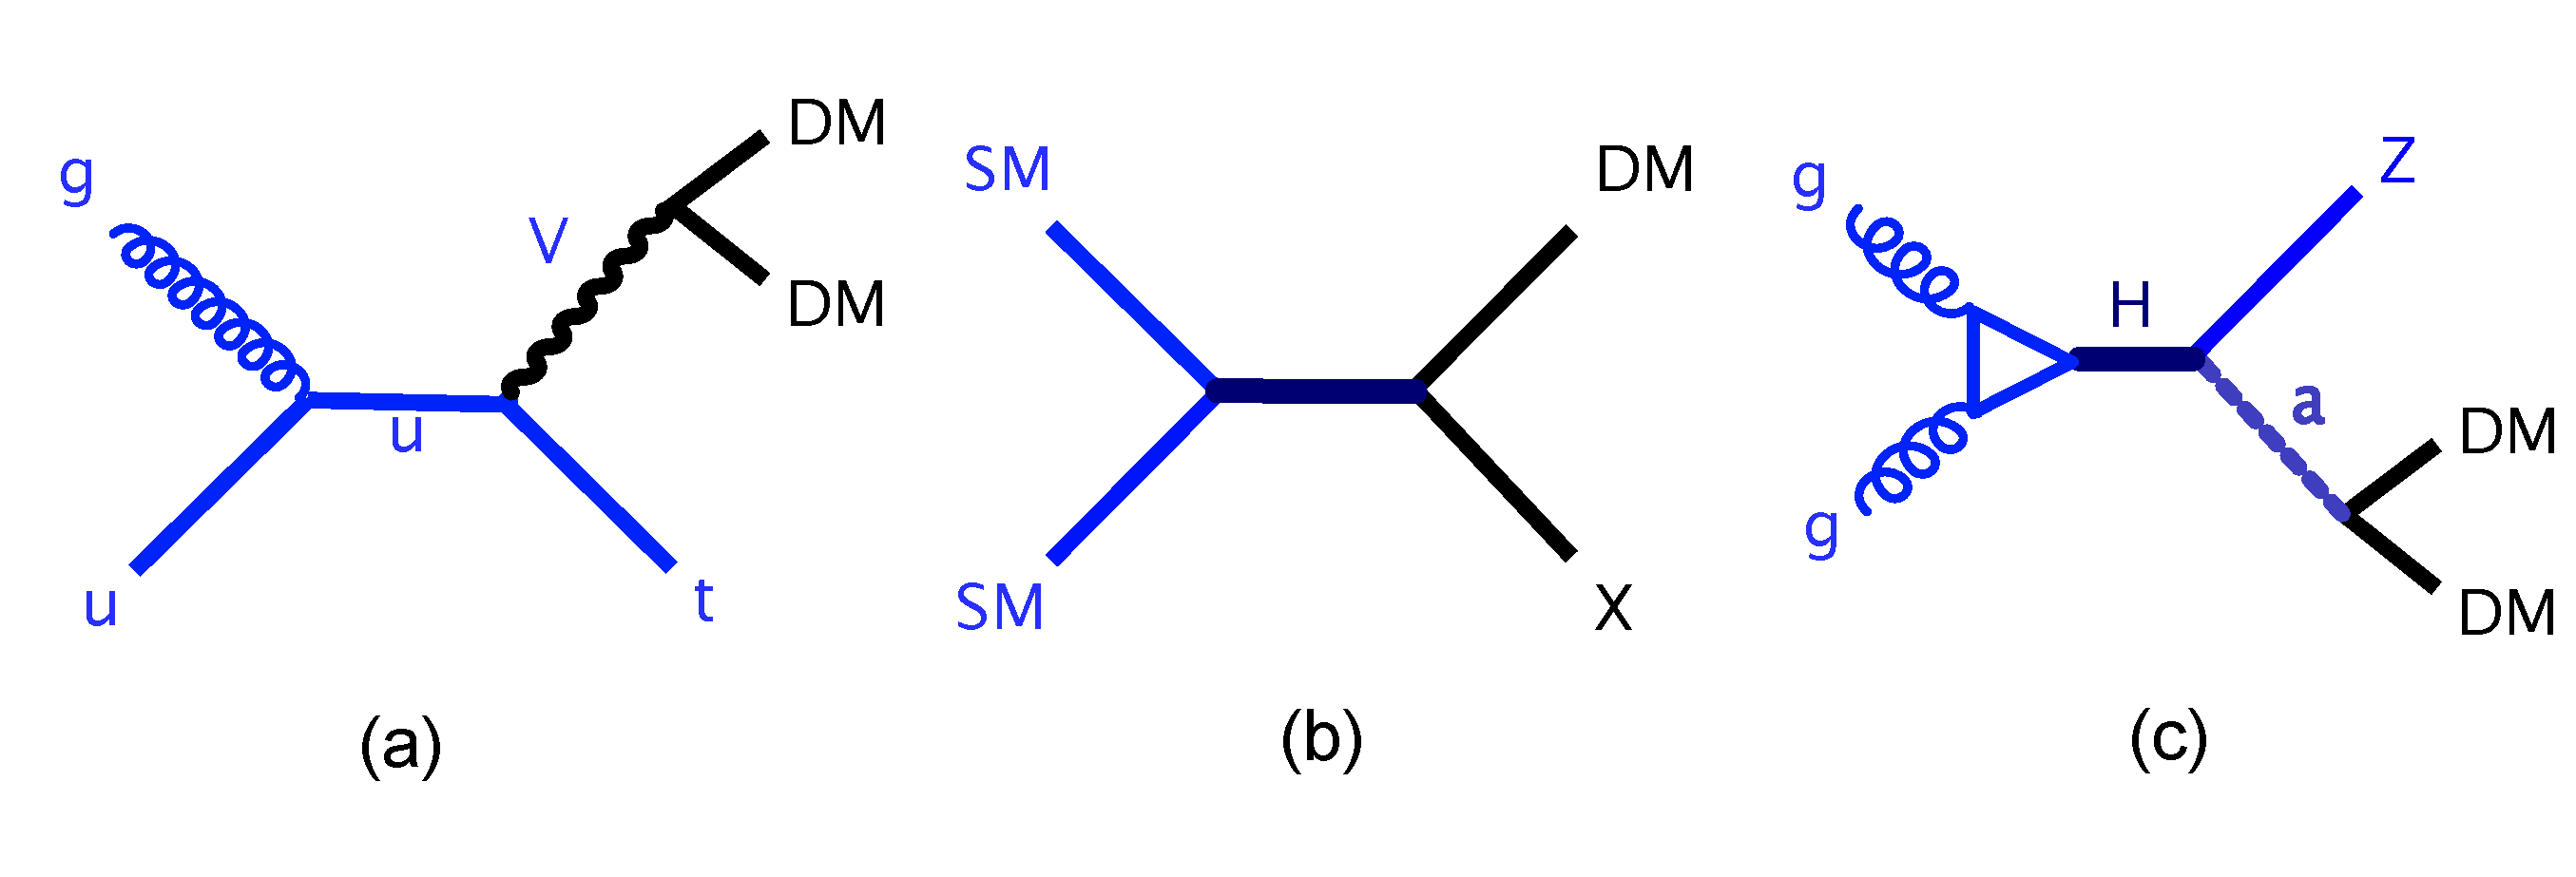
\includegraphics[width=\textwidth]{feynman_2}
%\caption{

(\textit{a}) Example of a process leading to a single top signature, proceeding through the coupling of a $u$ and a  $t$ with a new vector boson, decaying to DM particles. 
(\textit{b}) Example of a collider diagram from a coannihilation model, where two DM particles are present in the final state (one denoted DM and the other  $X$). 
(\textit{c}) Example of a diagram from a 2HDM process, with an interaction between an  $H$, an SM $Z$ boson, and an $a$ mediating the SM--DM interaction. 
Abbreviations:\ $a$, pseudoscalar boson; DM, dark matter; $g$, gluon; $H$, heavy Higgs boson; SM, Standard Model; $t$, top quark;  $u$, up quark; $V$, vector mediator; $X$, coannihilating DM partner, 2HDM, two--Higgs doublet model.

%\label{fig:feynman_2}
%}
%\end{figure}